\section{Quaternion}
\hspace{\parindent}\footnote{\href{https://faculty.sites.iastate.edu/jia/files/inline-files/quaternion.pdf}{Here's} the source for this note.}Quaternion $q$ is a sum of a scalar $q_0$ and a vector $\boldsymbol q = (q_1, q_2, q_3)$, namely,
\begin{align}
    q = q_0 + \boldsymbol q = q_0 + q_1 \boldsymbol{\hat i} + q_2 \boldsymbol{\hat j} + q_3 \boldsymbol{\hat k}.
    \label{eqn:quaternion}
\end{align}

The products of the quaternion satisfy the following rules developed by Hamilton; the rules are what allow for rotational operations using quaternions. In other words, these rules are central for the ``rotational math" to work.
\begin{align}
    \boldsymbol{\hat i} \otimes \boldsymbol{\hat i} = \boldsymbol{\hat j} \otimes \boldsymbol{\hat j} = \boldsymbol{\hat k} \otimes \boldsymbol{\hat k} = -1
    \label{eqn:quaternionProductRules}
\end{align}

The product of $2$ quaternions, $p = p_0 + \boldsymbol p$ and $q = q_0 + \boldsymbol q$, can be compactly represented as
\begin{align}
    p \otimes q = p_0 q_0 - \boldsymbol p \cdot \boldsymbol q + p_0 \boldsymbol q + q_0 \boldsymbol p + \boldsymbol p \times \boldsymbol q,
    \label{eqn:quaternionProduct}
\end{align}
where $\boldsymbol{p}, \boldsymbol{q} \in\Re^{3}$ are vector part of the quaternions $p$, and $q$, respectively.

Before diving into how quaternions are used to describe rotations, let's look go through the definitions of norm, conjugate, and inverse of quaternion.
\begin{itemize}
    \item \textit{Conjugate}: The conjugate of the quaternion $q = q_0 + \boldsymbol{q}$ is defined as $q^* = q_0 - \boldsymbol{q}$
    \item \textit{Norm}: The norm of the quaternion $q = q_0 + \boldsymbol{q}$ is defined as $|q| = \sqrt{q \otimes q^*}$. Quaternion whose norm is $1$ is a unit quaternion; unit quaternions are what are used for pure rotation, i.e., without scaling of the vectors
    \item \textit{Inverse}: The inverse of the quaternion $q = q_0 + \boldsymbol{q}$ is defined as $q^{-1} = \frac{q^*}{|q|^2}$
\end{itemize}
%----------------------------------------------------------------------------

%----------------------------------------------------------------------------
\subsection{Rotation Operator}
\hspace{\parindent}A vector $\boldsymbol{v} \in\Re^3$ is also a quaternion without the real part; quaternion whose real part is $0$ is called a \textit{pure quaternion}. Let's define a linear operator (not a rotation operator) that acts on $\boldsymbol{v} \in\Re^3$ as
\begin{align}
    L_q(\boldsymbol{v}) \triangleq q \otimes \boldsymbol{v} \otimes q^*.
    \label{eqn:LOperator}
\end{align}

Now let's focus on just the rotation.

\paragraph{Theorem 1}Let
\begin{align}
    \hat q = q_0 + \boldsymbol{q} = \cos{\frac{\theta}{2} + \boldsymbol{\hat u} \sin{\frac{\theta}{2}}}
    \label{eqn:unitQuaternion}
\end{align}
be a unit quaternion. Then, the action of the operator $L_{\hat q}$ on a vector $\boldsymbol{v} \in\Re^3$ is equivalent to a rotation of $\boldsymbol{v}$ about $\boldsymbol{\hat u}$ axis by $\theta$ amount. Note that $\boldsymbol{\hat u}$ is a unit vector.

\paragraph{Proof} Let the vector $\boldsymbol{v} = \boldsymbol{a} + \boldsymbol{n}$, where $\boldsymbol{a} \in\Re^3$ and $\boldsymbol{n} \in\Re^3$ are the components of $\boldsymbol{v} \in\Re^3$ that are parallel and perpendicular to $\boldsymbol{u}$, respectively; $\boldsymbol{u} \in\Re^3$ is the imaginary part of the quaternion $q$.

The action of the operator $L_{\hat q}$ on $\boldsymbol{a}$ is invariant, i.e.,
\begin{align}
    L_{\hat q}(\boldsymbol{a}) = \boldsymbol{a}.
    \label{eqn:rotationOperationOnParallelComponent}
\end{align}

Whereas, the action of the operator $L_{\hat q}$ on $\boldsymbol{n}$ is
\begin{align}
    L_{\hat q}(\boldsymbol{n}) &= (q_0^2 - ||\boldsymbol{q}||^2) \boldsymbol n + 2 q_0 ||\boldsymbol{q}|| (\boldsymbol{\hat u} \times \boldsymbol{n}),
    \label{eqn:rotationOperationOnPerpendicularComponent1}
\end{align}
and after introducing $\boldsymbol{n}_{\perp} = \boldsymbol{\hat u} \times \boldsymbol{n}$ and noting $\boldsymbol{\hat u} = \frac{\boldsymbol{q}}{||\boldsymbol{q}||}$, we get
\begin{align}
    L_{\hat q}(\boldsymbol{n}) &= (q_0^2 - ||\boldsymbol{q}||^2) \boldsymbol n + 2 q_0 ||\boldsymbol{q}|| \boldsymbol{n}_{\perp}.
    \label{eqn:rotationOperationOnPerpendicularComponent2}
\end{align}

Since $\boldsymbol{\hat u}$ is a unit vector, $||\boldsymbol{n}_\perp|| = ||\boldsymbol{\hat u} \times \boldsymbol{n}|| = ||\boldsymbol{n}||$. After substituting for $q_0$ and $||\boldsymbol{q}||$ from Eq.~\ref{eqn:unitQuaternion} to Eq.~\ref{eqn:rotationOperationOnPerpendicularComponent2}, we get
\begin{align}
    L_{\hat q}(\boldsymbol{n}) &= \left( \cos^2{\frac{\theta}{2}} - \sin^2{\frac{\theta}{2}} \right) \boldsymbol{n} + \left( 2 \cos{\frac{\theta}{2}} \sin{\frac{\theta}{2}} \right) \boldsymbol{n}_\perp, \\
    &= \cos{\theta} \boldsymbol{n} + \sin{\theta} \boldsymbol{n}_\perp.
    \label{eqn:rotationOperationOnPerpendicularComponent3}
\end{align}

Eq.~\ref{eqn:rotationOperationOnPerpendicularComponent3} tells us that the action of $L_{\hat q}$ on $\boldsymbol{n}$ is a rotation of $\boldsymbol{n}$ by $\theta$ amount. Since, $\boldsymbol{n}$ is perpendicular to $\boldsymbol{\hat u}$, and the tail of $\boldsymbol{n}$ intersects the axis of $\boldsymbol{\hat u}$, the axis of rotation is also the axis of $\boldsymbol{\hat u}$. Fig.~\ref{fig:resultOfLOnV} depicts the action of $L_{\hat q}$ on $\boldsymbol{n}$, and $\boldsymbol{v}$.

\begin{figure}[h]
\centering
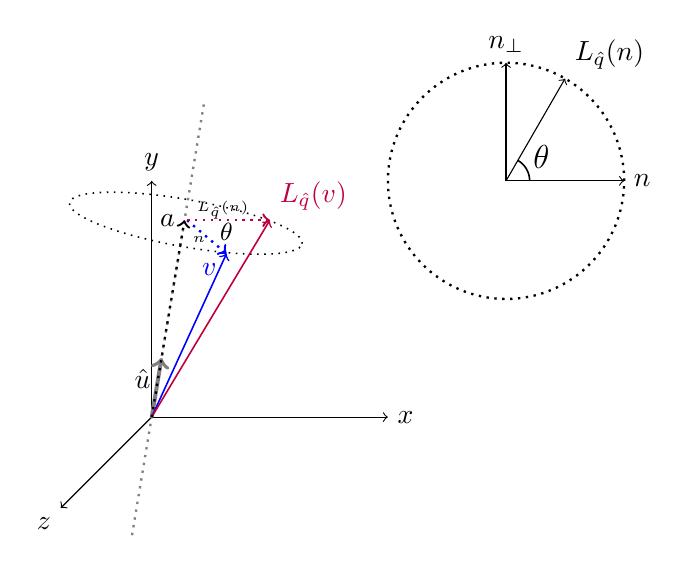
\begin{tikzpicture}
    % Draw the 3D axes
    \draw[->] (0,0,0) -- (3,0,0) node[right] {$x$};
    \draw[->] (0,0,0) -- (0,3,0) node[above] {$y$};
    \draw[->] (0,0,0) -- (0,0,3) node[below left] {$z$};

    % Define arbitrary axis of rotation
    \draw[->, line width=0.5mm, gray] (0,0,0) -- (0.125,0.75,0) node[below left] {\textcolor{black}{$\boldsymbol{\hat{u}}$}};
    \draw[dotted, line width=0.3mm, gray] (-0.25,-1.5,0) -- (0.6667,4,0);

    % Rotation arc
    \draw[dotted, line width=0.2mm, rotate=-10] (0,2.5,0) ellipse (1.5cm and 0.3cm);

    % Initial vector before rotation
    \draw[->, line width=0.2mm, blue] (0,0,0) -- (0.95,2.075,0) node[below left] {$\boldsymbol{v}$};
    % Rotated vector after rotation
    \draw[->, line width=0.2mm, purple] (0,0,0) -- (1.5,2.5,0) node[above right] {$L_{\hat q}(\boldsymbol{v})$};

    % Perpendicular component
    \draw[dotted, ->, line width=0.3mm, blue] (0.45,2.5,0) -- (.95,2.075,0);
    \draw[dotted, ->, line width=0.3mm, purple] (0.45,2.5,0) -- (1.5,2.5,0);
    % Parallel component
    \draw[dotted, ->, line width=0.3mm] (0,0,0) -- (0.41667,2.5,0) node at (0.2,2.5) {$\boldsymbol{a}$};

    % Angle Subtended
    \node at (0.95,2.35) [font=\fontsize{9}{0.5}] {$\theta$};
    % \draw[line width=0.2mm] (0.75,2.25,0) arc[start angle=-10, end angle=20, radius=5mm];

    % Maybe this is too much
    % Miniaturized perpendicular components
    \node at (0.6,2.25) [font=\fontsize{0.5}{0.5}] {$\boldsymbol{n}$};
    \node at (0.9,2.625) [font=\fontsize{0.5}{0.5}] {$L_{\hat q}(\boldsymbol{n})$};

    % Zoomed-in content inside the circle
    \begin{scope}[scale=1.5, shift={(3, 2)}]
        % Rotation path
        \draw[dotted, line width=0.3mm, black] (0,0) circle(1);

        % Parallel and perpendicular components of n
        \draw[->] (0,0,0) -- (1,0,0) node[right] {$\boldsymbol{n}$};
        \draw[->] (0,0,0) -- (0,1,0) node[above] {$\boldsymbol{n}_\perp$};

        % n after the operator action
        \draw[->] (0,0,0) -- (0.5,0.866,0) node[above right] {$L_{\hat q}(\boldsymbol{n})$};

        % Angle Subtended
        \node at (0.3,0.2, 0) [font=\fontsize{12}{0.5}] {$\theta$};
        \draw[line width=0.2mm] (0.2,0,0) arc[start angle=0, end angle=60, radius=2mm];
    \end{scope}

\end{tikzpicture}

\caption{The result of the action of the operator $L_{\hat q}$ on the vector $\boldsymbol{v}$. The component of $\boldsymbol{v}$ that is perpendicular to $\boldsymbol{\hat u}$, i.e., $\boldsymbol{n}$, before and after the action of the operator $L_{\hat q}$ are color-coded and shown by the dotted arrows. $\boldsymbol{a}$ is the parallel component which is invariant to the operator $L_{\hat q}$. Note that the dotted ellipse is infact a circle since the operator takes a unit quaternion to act on the vector in this illustration. On the scaled portion, $\boldsymbol{n}_\perp$ is perpendicular to $\boldsymbol{n}$ and both $\boldsymbol{q}$, and $\boldsymbol{\hat u}$ point out of the screen from the origin.}
\label{fig:resultOfLOnV}
\end{figure}

To summarize, Eq.~\ref{eqn:rotationOperationOnParallelComponent} \& \ref{eqn:rotationOperationOnPerpendicularComponent3} along with Fig.~\ref{fig:resultOfLOnV} tell us that the action of the linear operator $L_{\hat q}$ on $\boldsymbol{v}$ is rotation of $\boldsymbol{v}$ by $\theta$ amount along the axis of $\boldsymbol{\hat u}$. For the sake of completeness, $L_{\hat q} = L_{-\hat q}$, i.e., $L_{\hat q}(\boldsymbol{v}) = L_{-\hat q}(\boldsymbol{v})$.
%----------------------------------------------------------------------------

%----------------------------------------------------------------------------
\subsection{Quaternion to Rotation Matrix}
\hspace{\parindent}Matrix representation for rotation can be obtained from the analysis of the linear operator $L_{\hat q}$ for a unit quaternion $\hat q$. Just a reminder that the linear operator can take any quaternion but only a unit quaternion can result in a pure rotation.

We know that $L_{\hat q}(\boldsymbol{v})$ rotates $\boldsymbol{v}$. To obtain the rotation matrix that rotates $\boldsymbol{v}$, we need to simplify the expression obtained from $L_{\hat q}(\boldsymbol{v})$ in a matrix-vector product form where the vector being multiplied by the matrix is $\boldsymbol{v}$; this implies that the matrix would be the rotation matrix.

Using the definition of the operator $L_{\hat q}$ from Eq.~\ref{eqn:LOperator} and the notation for the components of a unit quaternion from Eq.~\ref{eqn:unitQuaternion}, one obtains
\begin{align}
    L_{\hat q}(\boldsymbol{v}) = \underbrace{\left( \left( q_0^2 - ||\boldsymbol{q}||^2 \right) I_3 + 2 \boldsymbol{q} \boldsymbol{q}^T + 2 q_0 [\boldsymbol{q}]_{\times} \right)}_{\text{$3 \times 3$ matrix}} \boldsymbol{v} = R \boldsymbol{v}
    \label{eqn:LOperatorMatrixProduct}
\end{align}
where $[.]_{\times}$ is a skew-symmetric operator. Thus, the rotation matrix $R$ can be achieved from the unit quaternion $\hat q$ as shown in Eq.~\ref{eqn:LOperatorMatrixProduct}. Deriving a unit quaternion from the rotation matrix is a different story.

Note that the rotation matrix $R$ is independent of $\boldsymbol{v}$ and only depends on the unit quaternion $\hat q$. If $R$ were to be dependent on $\boldsymbol{v}$, one could still get the rotation matrix as long as the vector that the matrix multiplies were to be $\boldsymbol{v}$. Anyway, since that's not the case, let's not create a hypothetical problem.
%----------------------------------------------------------------------------

%----------------------------------------------------------------------------
\subsection{Rotation \& Coordinate Transformation}
\hspace{\parindent}\footnote{\href{https://sites.utexas.edu/near/files/2022/07/Rotations.pdf}{Here's} the source for rotation, coordinate transformations, left quaternions, right quaternions?}Next, we explore \textit{active} and \textit{passive} rotations. After going through the \href{https://sites.utexas.edu/near/files/2022/07/Rotations.pdf}{article}, the information I found ``useful", subjectively, to me at the moment of writing this section of the note is as follows:
\begin{itemize}
    \item \textit{Active Rotation}: Attitude of a rigid-body can be expressed as the rotation from an inertial frame to a body-fixed frame. Let $R_{i \rightarrow b}$ be the rotation matrix that rotates an inertial frame into the body-fixed frame. This representation of the attitude is called active rotation. In the active rotation, the observer is fixed to the inertial frame.
    \item \textit{Passive Rotation}: In the passive rotation, the observer is fixed to the body-fixed frame. Let $T_{b}^{i}$ be the coordinate transformation matrix, s.t., $\boldsymbol{v}^i = T_{b}^i \boldsymbol{v}^b$ where, $\boldsymbol{v}^b$ and $\boldsymbol{v}^b$ are the coordinates of the vector $\boldsymbol{v}$ in the body-fixed and inertial frames, respectively.
\end{itemize}

Note that $T_{i}^b = R_{i \rightarrow b}^{T}$. Essentially, the active and passive rotation matrices are related in the same way as the rotation and orientation matrices are related to each other.

We already know how to compose the rotation and coordinate transformation matrices. Here's the summary of the compositions for completeness.
\begin{itemize}
    \item $R_{i \rightarrow c} = R_{i \rightarrow b} R_{b \rightarrow c}$, where the successive rotations are referenced to the body-fixed frame, a.k.a., rotating frame. If the rotations are referenced to the inertial frame, then the order is flipped.
    \item $T_{c}^i = T_{b}^i T_{c}^b$.
\end{itemize}

The composition rules for the rotation matrices above were something we were already familiar with. Our goal is to find how the quaternion representations of the attitude are composed. The \href{https://sites.utexas.edu/near/files/2022/07/Rotations.pdf}{article} mentions Hamilton's product ($\circledast$) and Shuster's product ($\otimes$) for quaternions. Shuster's product is defined in a way that allows us to write the successive composition of quaternions referenced to the rotating frame in the same order as ``transformation" matrix. We'll skip Shuster's product because it's just another definition that is introduced such that quaternions can be multiplied in order. There's no need to multiply quaternions in the ``same order" as the corresponding matrix multiplication.

First, let's \textcolor{blue}{define ``$\otimes$" as Hamilton's product} to remain consistent with this note. Unlike the Shuster's product, the composition of successive rotations referenced to the rotating frame follows the same order as the matrix multiplication.
\begin{itemize}
    \item For the successive rotations relative to the rotating frame, let $\hat{q}_{i \rightarrow b}$ and $\hat{q}_{b \rightarrow c}$ be the quaternion representations of the rigid-body rotations in succession. Then, the composition is
    \begin{align}
        \hat{q}_{i \rightarrow c} = \hat{q}_{i \rightarrow b} \otimes \hat{q}_{b \rightarrow c}.
    \end{align}
    \item For the vector (and point) coordinates transformation, one first constructs a \textit{pure} quaternion of the vector or point and applies the operator in Eq.~\ref{eqn:LOperator} as
    \begin{align}
        \begin{bmatrix}
            0 \\
            \boldsymbol{v}^i
        \end{bmatrix}
        =
        \hat{q}_{i \rightarrow b}
        \begin{bmatrix}
            0 \\
            \boldsymbol{v}^b
        \end{bmatrix}
        \hat{q}^{*}_{i \rightarrow b}
    \end{align}
    where $({}^*)$ represents conjugate of the quaternion. Note that the conjugate premultiplies the vector.
    \item Tying this section to the previous sections of this note, if one wants to rotate the vector (not coordinate transformation), then the operator in Eq.~\ref{eqn:LOperator} is applied as
    \begin{align}
        \begin{bmatrix}
            0 \\
            \boldsymbol{v}'
        \end{bmatrix}
        =
        \hat{q}
        \begin{bmatrix}
            0 \\
            \boldsymbol{v}
        \end{bmatrix}
        \hat{q}^* .
    \end{align}
\end{itemize}
%----------------------------------------------------------------------------